\documentclass{article}

\usepackage{amsmath} % Used for mathematical formulas
\usepackage{graphicx} % Used for inserting images
\usepackage{lipsum} % Used for generating placeholder text
\usepackage{ctex} % Imported the ctex package to support Chinese
\usepackage{titlesec} % Imported the titlesec package for customizing title styles
\usepackage{fontspec} % Used for setting Chinese fonts

\setmainfont{SimSun} % Set the Chinese font to SimSun (宋体 system font)

\usepackage{listings}
\usepackage{color}
\usepackage{float}

\title{实验报告:数据流工具}
\author{程智镝}
\date{\today}

\begin{document}

\maketitle

\section*{涵盖工具}

本实验涵盖以下数据流工具:

\begin{enumerate}
    \item Apache Kafka
    \item AWS Kinesis
    \item Apache NiFi
    \item Flume
\end{enumerate}

\section*{实验任务}

\begin{enumerate}
    \item 任务一:使用 Apache Kafka 进行数据流
    \begin{itemize}
        \item \textbf{要求:}安装 Apache Kafka。
        \item \textbf{任务:}生产和消费一个简单的消息。
        \item \textbf{验证:}确认 Kafka 主题中的消息。
    \end{itemize}
    
    \item 任务二:使用 AWS Kinesis 进行实时数据摄取
    \begin{itemize}
        \item \textbf{要求:}在 AWS 控制台中创建一个 Kinesis 流。
        \item \textbf{任务:}使用 AWS SDK 发送一批消息。
        \item \textbf{验证:}在 Kinesis 控制台中监控传入数据。
    \end{itemize}
    
    \item 任务三:使用 Apache NiFi 进行数据流管理
    \begin{itemize}
        \item \textbf{要求:}安装 Apache NiFi。
        \item \textbf{任务:}创建一个简单的数据流,将数据从平面文件移动到数据库。
        \item \textbf{验证:}确认数据库中的记录。
    \end{itemize}
    
    \item 任务四:使用 Flume 收集日志
    \begin{itemize}
        \item \textbf{要求:}安装 Flume。
        \item \textbf{任务:}配置 Flume 以收集日志并将其存储在 HDFS 中。
        \item \textbf{验证:}确认 HDFS 中存储的日志。
    \end{itemize}
\end{enumerate}

\section*{实验难点}

\begin{itemize}
    \item 未使用过该配置
    \item 构造数据
    \item 我使用的是阿里云而不是 AWS,配置上可能会有差距
\end{itemize}

\section*{任务一}

\textbf{任务流程参照:}\verb|https://blog.csdn.net/sun_hong_likeIT/article/details/123502688|

下载 Apache Kafka:\texttt{sudo wget https://mirrors.tuna.tsinghua.edu.cn/apache/kafka/3.5.1/kafka\_2.12-3.5.1.tgz}

这里使用的是清华镜像网站,比教程给的网站更好用。

使用 \texttt{bin/zookeeper-server-start.sh -daemon config/zookeeper.properties} 以守护进程启动)

启动 Kafka:\texttt{bin/kafka-server-start.sh config/server.properties \&}

新建终端创建主题:\texttt{bin/kafka-topics.sh --bootstrap-server localhost:9092 --create --topic test --partitions 2 --replication-factor 1}

在主题终端发送消息:\texttt{bin/kafka-console-producer.sh --broker-list localhost:9092 --topic test}

服务终端接收到消息:\texttt{bin/kafka-console-consumer.sh --bootstrap-server localhost:9092 --topic test --from-beginning}

消息生产和消费过程:
\begin{figure}[htbp]
    \centering
    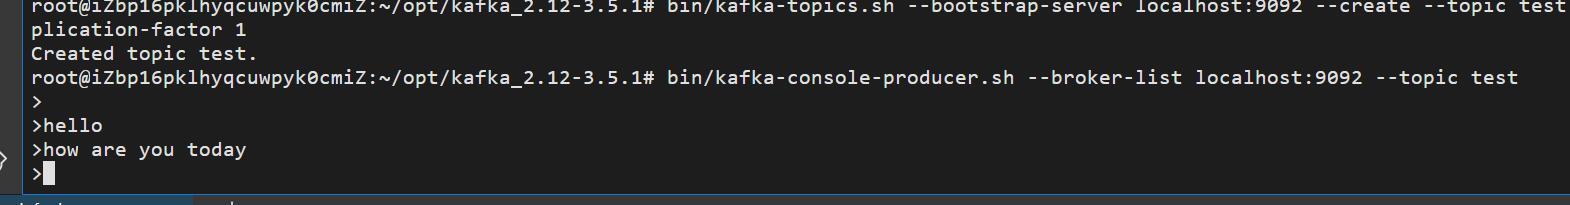
\includegraphics{mission1.1.jpg}
    \includegraphics*{mission1.2.jpg}
    \caption{Elliptic Paraboloid}
\end{figure}

\section*{任务二}

由于我使用的不是 AWS,我在阿里云上使用了数据总线来进行平替:https://www.aliyun.com/product/bigdata/datahub

\section*{任务三}

\textbf{步骤一:}\\
NiFi 安装:\texttt{wget https://mirrors.tuna.tsinghua.edu.cn/apache/nifi/1.23.2/nifi-1.23.2-bin.zip}

解压:\texttt{unzip nifi-1.23.2.zip}

提示:不知道为什么,网上大多数下载方法(使用镜像)我都无法成功下载,只能用官网的来下,真的巨慢……最后还是自己找了清华镜像自己wget,别看网上教程了\\

用官网会很慢,建议使用国内镜像\\
\textbf{步骤二:}\\
配置 JAVA\_HOME, \texttt{sudo update-alternatives --config java} 这个指令可以快速帮你找到 java 路径。
\texttt{export JAVA\_HOME=你的 Java 所在的路径},比如我的就是 \texttt{/usr/lib/jvm/java-11-openjdk-amd64}

NiFi,启动!  \texttt{./bin/nifi.sh start}

\section*{任务四}
参考:https://www.cnblogs.com/j-y-s/p/16018612.html
安装 Flume:\texttt{wget https://mirrors.tuna.tsinghua.edu.cn/apache/flume/1.11.0/apache-flume-1.11.0-bin.tar.gz}
解压 \texttt{tar -zvxf 包名}
中途遇到了云实例不允许root使用密码登录,解决办法:VNC关防火墙:(sudo) ufw disable
云实例没办法使用jps指令:
修复dpkg:\texttt{sudo dpkg --configure -a}
安装:\texttt{sudo apt install openjdk-11-jdk-headless}
途中遇到了云实例连接超时的问题,网络上所有的关于配置ip白名单的都试过了,都没用,到最后还是因为防火墙没关,登录vnc,\texttt{sudo ufw disable}即可

\end{document}
